\section{Resultados}\label{sec:resultados}

\begin{table*}[t]
\centering
\caption{Média nas 6 cenas do Shiny Blender, treino só com vistas abaixo de 25°. Faixa e acima: vistas de teste; de cima: vistas de treino não usadas, entre 50° e 89°. As correções são aplicadas ao mesmo modelo treinado, sem novo treino. Em negrito, o melhor entre as variantes desse modelo.}
\label{tab:principal25}
\begin{tabular}{l ccc ccc ccc}
\toprule
 & \multicolumn{3}{c}{Dentro da faixa ($<25$°)} & \multicolumn{3}{c}{Acima (25°--47°)} & \multicolumn{3}{c}{De cima (50°--89°)} \\
\cmidrule(lr){2-4}\cmidrule(lr){5-7}\cmidrule(lr){8-10}
Variante & PSNR$\uparrow$ & SSIM$\uparrow$ & LPIPS$\downarrow$ & PSNR$\uparrow$ & SSIM$\uparrow$ & LPIPS$\downarrow$ & PSNR$\uparrow$ & SSIM$\uparrow$ & LPIPS$\downarrow$ \\
\midrule
3DGS (original) & \textbf{26{,}73} & 0{,}915 & 0{,}143 & 22{,}67 & 0{,}846 & 0{,}225 & 20{,}90 & 0{,}812 & 0{,}256 \\
Só termo constante (DC) & 24{,}98 & 0{,}905 & 0{,}166 & 22{,}53 & \textbf{0{,}854} & 0{,}223 & 20{,}93 & \textbf{0{,}821} & \textbf{0{,}246} \\
Projeção global & 26{,}71 & 0{,}916 & 0{,}143 & 22{,}89 & 0{,}852 & 0{,}219 & \textbf{21{,}03} & 0{,}816 & 0{,}249 \\
Projeção por visibilidade & 26{,}67 & \textbf{0{,}916} & \textbf{0{,}142} & \textbf{22{,}95} & 0{,}854 & \textbf{0{,}216} & 20{,}98 & 0{,}818 & 0{,}247 \\
\midrule
\textit{Referência: treino com o hemisfério todo} & 28{,}60 & 0{,}940 & 0{,}115 & 29{,}12 & 0{,}934 & 0{,}125 & n/a & n/a & n/a \\
\bottomrule
\end{tabular}
\end{table*}


\subsection{QP1: quanto se perde e quanto vale a cobertura}

A Fig.~\ref{fig:curva} mostra o PSNR médio das seis cenas em função da elevação da vista de avaliação. Dentro da faixa de treino, o 3DGS atinge 26,7~dB. Nas vistas de teste acima da faixa cai para 22,7~dB e nas vistas de cima, para 20,9~dB (Tabela~\ref{tab:principal25}): 5,8~dB perdidos apenas pela mudança de altura da câmera, com o LPIPS quase dobrando (de 0,143 para 0,256). A queda começa logo acima de 25° e continua até a vista de topo.

O modelo de referência, treinado com o hemisfério todo, mostra que a perda decorre da cobertura e não da dificuldade das vistas: com ele, as vistas acima de 25° atingem 29,1~dB, tanto quanto as de baixo (28,6~dB), enquanto o modelo da faixa fica em 22,7~dB nelas. Com treino abaixo de 15° (de 14 a 21 vistas por cena), a perda cresce: 22,7~dB na faixa, 19,0~dB acima e 17,4~dB de cima, e a distância até a referência acima da faixa passa de 6,5~dB para 10,2~dB. Para captura, isso quantifica o valor de cada grau adicional de elevação coberto.

\begin{figure}[t]
\centering
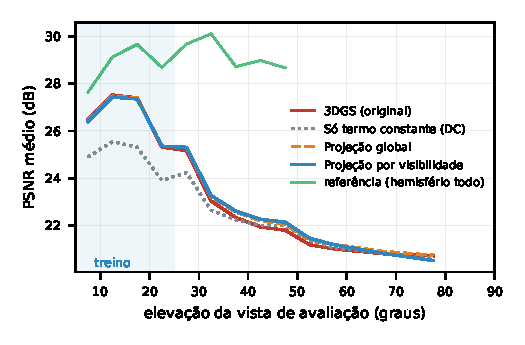
\includegraphics[width=\columnwidth]{figs/curva_elevacao_b25.pdf}
\caption{PSNR médio das seis cenas por elevação da vista de avaliação (intervalos de 5°), com treino só abaixo de 25° (área azul). Todas as variantes saem do mesmo modelo treinado; a linha verde é o modelo de referência, treinado com o hemisfério todo.}
\label{fig:curva}
\end{figure}

\subsection{QP2: oráculos mostram que cor e geometria se compensam}

\begin{table}[t]
\centering
\caption{PSNR (dB) fora da faixa de treino ($<25$°), nas vistas de índice ímpar de cada grupo. Oráculo: só a cor (SH) reajustada nas vistas de índice par do mesmo grupo, geometria congelada; é o teto de uma correção só de cor. Ref-G.: Ref-Gaussian treinado com as mesmas vistas.}
\label{tab:decomp25}
\setlength{\tabcolsep}{3pt}
\footnotesize
\begin{tabular}{l cccc cccc}
\toprule
 & \multicolumn{4}{c}{Acima} & \multicolumn{4}{c}{De cima} \\
\cmidrule(lr){2-5}\cmidrule(lr){6-9}
Cena & 3DGS & proj. & Ref-G. & oráculo & 3DGS & proj. & Ref-G. & oráculo \\
\midrule
\textit{ball} & 15{,}62 & 15{,}66 & 17{,}35 & 24{,}11 & 15{,}02 & 14{,}90 & 16{,}19 & 18{,}96 \\
\textit{car} & 21{,}68 & 21{,}72 & 22{,}93 & 27{,}24 & 19{,}64 & 19{,}48 & 20{,}92 & 26{,}05 \\
\textit{coffee} & 24{,}33 & 24{,}57 & 23{,}77 & 30{,}52 & 19{,}38 & 19{,}32 & 19{,}08 & 27{,}08 \\
\textit{helmet} & 22{,}33 & 22{,}61 & 22{,}65 & 28{,}89 & 21{,}29 & 21{,}45 & 20{,}75 & 27{,}08 \\
\textit{teapot} & 38{,}19 & 39{,}20 & 38{,}21 & 43{,}08 & 35{,}61 & 36{,}25 & 34{,}50 & 43{,}02 \\
\textit{toaster} & 13{,}90 & 13{,}98 & 17{,}33 & 20{,}06 & 14{,}86 & 14{,}90 & 16{,}19 & 20{,}14 \\
\midrule
Média & 22{,}68 & 22{,}96 & 23{,}71 & 28{,}98 & 20{,}97 & 21{,}05 & 21{,}27 & 27{,}05 \\
\bottomrule
\end{tabular}
\end{table}


O oráculo de cor, que reajusta todos os SH com a geometria congelada, eleva o PSNR de 21,0 para 27,1~dB de cima e de 22,7 para 29,0~dB acima (Tabela~\ref{tab:decomp25}), o nível da faixa filmada; a projeção fica longe desse teto. A Fig.~\ref{fig:qualitativo} mostra o efeito: mesmo com a cor ajustada apenas em vistas do lado oposto do objeto, a vista de 89° perde as manchas do 3DGS.

Os controles mudam a interpretação desse resultado (Tabela~\ref{tab:oraculos25}). Reajustar apenas a geometria, com a cor congelada, recupera ainda mais: 8,0~dB de cima. Reajustar apenas a cor constante recupera 4,1~dB. No controle mais rigoroso, com ajuste num lado do objeto e avaliação no outro, os ganhos caem para 2,3~dB (cor) e 3,1~dB (geometria), mas permanecem positivos. Cor e geometria, portanto, se substituem: a informação contida nas vistas de cima corrige a imagem por qualquer um dos dois caminhos. O modelo tem capacidade para representar a imagem correta; falta a informação.

\begin{table}[t]
\centering
\caption{Oráculos nas vistas de cima (PSNR em dB, treino abaixo de 25°). Cada oráculo reajusta só uma parte do modelo usando vistas de referência de cima: a cor constante de cada Gaussiana (DC), todos os SH (cor) ou posições, escalas, rotações e opacidades (geom.). Ímpares: ajuste nas vistas de índice par, avaliação nas ímpares. Lado oposto: ajuste num lado do objeto, avaliação no outro.}
\label{tab:oraculos25}
\setlength{\tabcolsep}{3pt}
\footnotesize
\begin{tabular}{l cccc ccc}
\toprule
 & \multicolumn{4}{c}{Ímpares} & \multicolumn{3}{c}{Lado oposto} \\
\cmidrule(lr){2-5}\cmidrule(lr){6-8}
Cena & 3DGS & DC & cor & geom. & 3DGS & cor & geom. \\
\midrule
\textit{ball} & 15{,}02 & 17{,}81 & 18{,}96 & 21{,}57 & 15{,}44 & 15{,}81 & 15{,}81 \\
\textit{car} & 19{,}64 & 23{,}87 & 26{,}05 & 27{,}22 & 19{,}56 & 22{,}90 & 23{,}79 \\
\textit{coffee} & 19{,}38 & 24{,}63 & 27{,}08 & 28{,}94 & 19{,}49 & 22{,}80 & 25{,}26 \\
\textit{helmet} & 21{,}29 & 24{,}50 & 27{,}08 & 27{,}74 & 21{,}37 & 22{,}50 & 23{,}03 \\
\textit{teapot} & 35{,}61 & 41{,}20 & 43{,}02 & 45{,}59 & 35{,}37 & 39{,}00 & 39{,}20 \\
\textit{toaster} & 14{,}86 & 18{,}31 & 20{,}14 & 22{,}49 & 15{,}04 & 17{,}08 & 17{,}51 \\
\midrule
Média & 20{,}97 & 25{,}06 & 27{,}05 & 28{,}92 & 21{,}04 & 23{,}35 & 24{,}10 \\
\bottomrule
\end{tabular}
\end{table}


\subsection{QP2: a geometria não piora de cima, mas está errada em todas as alturas}\label{sec:geometria}

O Shiny Blender fornece, para cada vista, a silhueta e o mapa de normais de referência, o que permite medir a geometria sem passar pela cor. Para cada vista de avaliação, renderizamos a opacidade acumulada e a profundidade esperada do modelo, derivamos as normais da profundidade (com suavização de 9~px) e as comparamos com a referência. Aplicado à profundidade de referência do conjunto, o mesmo cálculo erra entre 10° e 20°, limite imposto pela quantização da disparidade fornecida.

A Tabela~\ref{tab:geometria25} resume o resultado. A silhueta tem o mesmo IoU nos três grupos (0,91, 0,90 e 0,91). O erro das normais é alto em todos eles, de 54° a 63° em média: em objetos reflexivos, o 3DGS tende a imitar o reflexo com Gaussianas fora da superfície, e a profundidade resulta irregular. Esse erro é \emph{menor} de cima (53,8°) do que na faixa filmada (63,4°), provavelmente porque de cima predominam superfícies planas voltadas para a câmera. Uma segunda estimativa, sem suavização, confirma o quadro: tomando como normal o eixo mais curto de cada Gaussiana, composto por alfa, como no GaussianShader~\cite{jiang2024gshader}, o erro é de 55° na faixa, 48° acima e 41° de cima (Tabela~\ref{tab:normais25}).

\begin{table}[t]
\centering
\caption{Geometria medida contra a referência do Shiny Blender, treino abaixo de 25°: IoU da silhueta e erro angular médio (graus) das normais derivadas da profundidade renderizada. F: dentro da faixa; A: acima; C: de cima.}
\label{tab:geometria25}
\setlength{\tabcolsep}{4pt}
\footnotesize
\begin{tabular}{l ccc ccc}
\toprule
 & \multicolumn{3}{c}{IoU da silhueta$\uparrow$} & \multicolumn{3}{c}{Erro da normal (°)$\downarrow$} \\
\cmidrule(lr){2-4}\cmidrule(lr){5-7}
Cena & F & A & C & F & A & C \\
\midrule
\textit{ball} & 0{,}903 & 0{,}877 & 0{,}901 & 58{,}1 & 58{,}1 & 52{,}8 \\
\textit{car} & 0{,}925 & 0{,}957 & 0{,}967 & 63{,}2 & 59{,}7 & 55{,}7 \\
\textit{coffee} & 0{,}936 & 0{,}958 & 0{,}958 & 58{,}4 & 54{,}4 & 51{,}3 \\
\textit{helmet} & 0{,}957 & 0{,}953 & 0{,}961 & 66{,}9 & 62{,}1 & 53{,}7 \\
\textit{teapot} & 0{,}992 & 0{,}994 & 0{,}993 & 58{,}9 & 54{,}4 & 48{,}9 \\
\textit{toaster} & 0{,}741 & 0{,}665 & 0{,}674 & 74{,}9 & 69{,}0 & 60{,}6 \\
\midrule
Média & 0{,}909 & 0{,}901 & 0{,}909 & 63{,}4 & 59{,}6 & 53{,}8 \\
Treino completo$^\dagger$ & 0{,}939 & 0{,}965 & 0{,}984 & 58{,}3 & 57{,}0 & 52{,}5 \\
\bottomrule
\end{tabular}
\vspace{2pt}
{\scriptsize $^\dagger$ modelo treinado com as 100 vistas do hemisfério, média de 6 cenas (as vistas de cima fazem parte do treino dele).}
\end{table}


O modelo de referência separa duas componentes da geometria. Com vistas de cima no treino, a silhueta melhora (IoU de cima de 0,91 para 0,98) e a imagem também (+6,5~dB acima da faixa). A orientação da superfície, porém, praticamente não muda: o erro das normais de cima fica em 52,5°, contra 53,8° do modelo da faixa, embora essas vistas façam parte do treino dele. Um 3DGS que reproduz corretamente a imagem de cima também tem a superfície errada; no 3DGS, uma imagem correta não exige normal correta.

Junto com os oráculos, isso descreve o mecanismo. Em objetos reflexivos, o 3DGS não recupera a superfície em nenhuma altura, nem quando treinado com todas. Ele reproduz as vistas filmadas com uma geometria errada e uma cor dependente de vista que a compensa, e essa combinação só foi ajustada para as direções filmadas. De cima, a geometria não piora, mas a compensação deixa de valer.

\subsection{QP3: modelar a reflexão corrige a forma, não a aparência de cima}\label{sec:refgs}

O Ref-Gaussian~\cite{yao2025refgaussian} calcula o reflexo a partir da normal da superfície e de um único mapa de ambiente para a cena. Em princípio, isso permitiria reaproveitar o ambiente visto refletido numa parte do objeto para prever o reflexo de outra parte, vista de outro ângulo.

A geometria do Ref-Gaussian é de fato correta. Treinado com o hemisfério todo, ele erra as normais em 5,7° na faixa e 5,2° acima, na média das seis cenas, contra 41° a 63° do 3DGS conforme a estimativa e o grupo (Tabela~\ref{tab:normais25}). Treinado apenas na faixa, mantém a superfície correta também de cima: 11,6° de erro, contra 56,7° (profundidade) e 43,2° (eixo) do 3DGS nas mesmas três cenas.

\begin{table}[t]
\centering
\caption{Erro angular médio das normais (graus) contra a referência. No 3DGS, a normal é derivada da profundidade renderizada (prof.) ou é o eixo mais curto de cada Gaussiana, composto por alfa (eixo); no Ref-Gaussian, é a normal que o próprio modelo usa no sombreamento. Cada bloco usa só as cenas em que todos os seus modelos existem.}
\label{tab:normais25}
\setlength{\tabcolsep}{5pt}
\footnotesize
\begin{tabular}{l ccc}
\toprule
Modelo & Faixa & Acima & De cima \\
\midrule
\multicolumn{4}{l}{\textit{6 cenas}} \\
3DGS, faixa 25° (prof.) & 63{,}4 & 59{,}6 & 53{,}8 \\
3DGS, faixa 25° (eixo) & 54{,}5 & 48{,}0 & 40{,}8 \\
3DGS, hemisfério todo$^\dagger$ (prof.) & 58{,}3 & 57{,}0 & 52{,}5 \\
3DGS, hemisfério todo$^\dagger$ (eixo) & 54{,}9 & 49{,}9 & 43{,}4 \\
Ref-Gaussian, hemisfério todo & 5{,}7 & 5{,}2 & n/a \\
\midrule
\multicolumn{4}{l}{\textit{6 cenas}} \\
3DGS, faixa 25° (prof.) & 63{,}4 & 59{,}6 & 53{,}8 \\
3DGS, faixa 25° (eixo) & 54{,}5 & 48{,}0 & 40{,}8 \\
Ref-Gaussian, faixa 25° & 11{,}0 & 11{,}6 & 11{,}0 \\
\bottomrule
\end{tabular}
\vspace{2pt}
{\scriptsize $^\dagger$ as vistas de cima fazem parte do treino deste modelo.}
\end{table}


\textbf{Imagem.} Treinado só na faixa, o Ref-Gaussian melhora a imagem em todas as alturas, mas a vantagem diminui com a elevação: +2,1~dB na faixa (24,5 contra 22,3~dB nas mesmas três cenas), +1,7~dB acima e +0,7~dB de cima (19,3 contra 18,6~dB). No \textit{helmet}, fica abaixo do 3DGS de cima (20,6 contra 21,2~dB). Da faixa para cima, o Ref-Gaussian perde 5,2~dB e o 3DGS, 3,7~dB. A comparação é equilibrada em treino: o Ref-Gaussian da faixa usa 28 mil iterações, e o 3DGS, 30 mil. A Fig.~\ref{fig:qualitativo} mostra que, de cima, o Ref-Gaussian não apresenta os riscos brancos do 3DGS, mas a pintura e o metal saem borrados.

\textbf{A informação existe, e não são as iterações.} Treinado com o hemisfério todo, o mesmo método atinge, acima da faixa, 30,8~dB nessas três cenas, contra 21,0~dB do treinado só na faixa. O modelo completo usa o cronograma original de 50 mil iterações, e por isso avaliamos também seus \textit{checkpoints} intermediários (Tabela~\ref{tab:refgsiter25}). Com 30 mil iterações, ele já atinge 31,1~dB acima da faixa nessas cenas, e na média das seis cenas a diferença entre 30 e 50 mil iterações é de 0,05~dB (de $-$0,9 a +0,5~dB por cena; no \textit{helmet} e no \textit{toaster}, 30 mil é melhor). A distância de cerca de 10~dB entre o modelo da faixa e o completo vem, portanto, das vistas de cima, e não do treino mais longo.

\begin{table}[t]
\centering
\caption{Ref-Gaussian nas vistas de teste acima de 25° (PSNR em dB): treinado só na faixa, com 28 mil iterações, contra o modelo treinado com todas as alturas avaliado nos \textit{checkpoints} de 30, 40 e 50 mil iterações. A diferença entre as colunas do modelo completo mede o efeito das iterações; a diferença para a primeira coluna, o efeito das vistas de cima.}
\label{tab:refgsiter25}
\setlength{\tabcolsep}{4pt}
\footnotesize
\begin{tabular}{l c ccc}
\toprule
 & Faixa & \multicolumn{3}{c}{Todas as alturas} \\
\cmidrule(lr){2-2}\cmidrule(lr){3-5}
Cena & 28 mil & 30 mil & 40 mil & 50 mil \\
\midrule
\textit{ball} & -- & 35{,}46 & 35{,}66 & 35{,}92 \\
\textit{car} & 22{,}90 & 31{,}60 & 31{,}91 & 32{,}07 \\
\textit{coffee} & -- & 33{,}81 & 33{,}97 & 34{,}10 \\
\textit{helmet} & 22{,}63 & 33{,}32 & 34{,}01 & 32{,}41 \\
\textit{teapot} & -- & 48{,}42 & 48{,}47 & 48{,}56 \\
\textit{toaster} & 17{,}30 & 28{,}25 & 28{,}68 & 28{,}05 \\
\midrule
Média (3 cenas) & 20{,}95 & 31{,}05 & 31{,}53 & 30{,}84 \\
\bottomrule
\end{tabular}
\end{table}


\textbf{O ambiente refletido de cima já foi observado.} Para cada pixel do objeto, calculamos a direção refletida com a normal de referência e marcamos, numa grade da esfera com células de 5°, as direções que aparecem nas vistas de treino. Em todas as seis cenas, 100\% das direções refletidas nas vistas de cima já aparecem em alguma vista de treino; no \textit{car}, no \textit{helmet} e no \textit{ball}, com a mesma densidade das vistas da faixa. Superfícies curvas refletem quase a esfera inteira de qualquer ponto de vista. Para um modelo com mapa de ambiente compartilhado, a informação sobre a iluminação de cima está disponível.

\textbf{O que falta: oráculos por componente.} Para identificar a parte da aparência que falha, aplicamos ao Ref-Gaussian o mesmo protocolo de oráculos do 3DGS: com a geometria congelada, reajustamos com as vistas de cima de índice par apenas o material (cor base, cor difusa, intensidade do reflexo, rugosidade e metalicidade de cada Gaussiana), apenas o mapa de ambiente, apenas a luz indireta aprendida, ou as três partes, e avaliamos nas vistas de índice ímpar (1000 passos de Adam com as taxas do treino). A Tabela~\ref{tab:refgsoraculos25} resume o resultado. O material é a componente que mais recupera: +1,6~dB em média, contra +0,6~dB do mapa de ambiente e +0,2~dB da luz indireta. Isso concorda com o teste de cobertura: o ambiente foi observado; o que não foi observado é como cada superfície voltada para cima reflete. Com câmeras abaixo de 25°, uma superfície horizontal só é vista a mais de 65° da sua normal, e sua rugosidade e intensidade de reflexo são ajustadas apenas nesses ângulos rasantes.

\begin{table*}[t]
\centering
\caption{Oráculos de cima, treino abaixo de 25° (PSNR em dB nas vistas de cima de índice ímpar; o ajuste usa as de índice par). No 3DGS, reajusta-se só a cor (SH) ou só a geometria. No Ref-Gaussian, reajusta-se só o material (cor base, cor difusa, intensidade do reflexo, rugosidade, metalicidade), só o mapa de ambiente, só a luz indireta, as três (aparência), só a geometria (posições, formas, opacidades e normais) ou tudo. No \textit{ball} há apenas cinco vistas de avaliação.}
\label{tab:refgsoraculos25}
\setlength{\tabcolsep}{4pt}
\footnotesize
\begin{tabular}{l ccc ccccccc}
\toprule
 & \multicolumn{3}{c}{3DGS} & \multicolumn{7}{c}{Ref-Gaussian} \\
\cmidrule(lr){2-4}\cmidrule(lr){5-11}
Cena & orig. & cor & geom. & orig. & material & ambiente & indireta & aparência & geometria & tudo \\
\midrule
\textit{ball} & 15{,}02 & 18{,}96 & 21{,}57 & 16{,}19 & 18{,}70 & 16{,}75 & 16{,}20 & 20{,}22 & 21{,}00 & 23{,}32 \\
\textit{car} & 19{,}64 & 26{,}05 & 27{,}22 & 20{,}92 & 23{,}08 & 21{,}71 & 20{,}94 & 23{,}73 & 26{,}94 & 27{,}87 \\
\textit{coffee} & 19{,}38 & 27{,}08 & 28{,}94 & 19{,}08 & 23{,}22 & 19{,}30 & 19{,}17 & 23{,}56 & 27{,}45 & 27{,}87 \\
\textit{helmet} & 21{,}29 & 27{,}08 & 27{,}74 & 20{,}75 & 22{,}08 & 21{,}40 & 21{,}17 & 23{,}58 & 27{,}28 & 28{,}21 \\
\textit{teapot} & 35{,}61 & 43{,}02 & 45{,}59 & 34{,}51 & 35{,}14 & 35{,}27 & 34{,}62 & 37{,}48 & 41{,}37 & 42{,}34 \\
\textit{toaster} & 14{,}86 & 20{,}14 & 22{,}49 & 16{,}19 & 17{,}46 & 16{,}68 & 16{,}32 & 18{,}56 & 22{,}16 & 23{,}08 \\
\midrule
Média (6) & 20{,}97 & 27{,}05 & 28{,}92 & 21{,}27 & 23{,}28 & 21{,}85 & 21{,}40 & 24{,}52 & 27{,}70 & 28{,}78 \\
\bottomrule
\end{tabular}
\end{table*}


Mesmo reajustando toda a aparência, porém, o Ref-Gaussian recupera apenas 2,7~dB de cima, contra 5,8~dB do oráculo de cor do 3DGS. A aparência do Ref-Gaussian é restrita pela física: a cor é calculada a partir da normal e do mapa de ambiente, e não pode compensar livremente uma geometria imperfeita, como os SH do 3DGS fazem. A geometria residual pesa mais nesse caso, porque o reflexo amplifica o erro de orientação: num espelho, uma normal desviada de $\theta$ desvia a direção refletida de $2\theta$, e os 11,6° de erro de normal de cima podem deslocar o reflexo em mais de 20°. A restrição física que dá ao Ref-Gaussian uma geometria correta é a mesma que o impede de compensar, pela aparência, o que falta de cima.

\begin{figure*}[t]
\centering
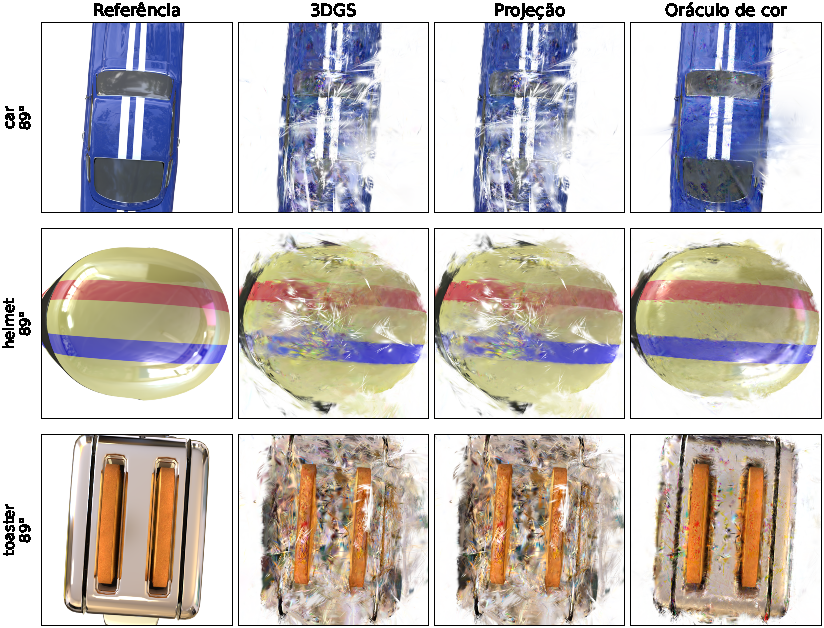
\includegraphics[width=0.8\textwidth]{figs/qualitativo_cima.pdf}
\caption{A vista mais alta de cada cena (89°), com treino só abaixo de 25°. A projeção remove pouco das manchas do 3DGS. No oráculo de cor, a geometria é a mesma e só a cor foi reajustada, em vistas de cima do lado oposto do objeto; esta vista não entrou no ajuste. O Ref-Gaussian, treinado nas mesmas vistas, tem a superfície correta, mas a aparência de cima continua borrada.}
\label{fig:qualitativo}
\end{figure*}

\subsection{QP4: a projeção é segura na faixa, mas recupera pouco}

\textbf{Dentro da faixa.} As duas projeções mudam o PSNR em menos de 0,1~dB (0,02~dB a global e 0,06~dB a por visibilidade), como prevê a garantia da Seção~\ref{sec:metodo}, e o LPIPS melhora ligeiramente. Descartar toda a dependência de vista (grau 0) custa 1,8~dB: os reflexos observados pelas câmeras são reais e precisam ser mantidos.

\textbf{Acima da faixa.} A projeção por visibilidade ganha 0,28~dB em média. O intervalo de confiança de 95\% por \textit{bootstrap} nas 642 vistas vai de 0,25 a 0,31~dB, e 84\% das vistas melhoram. Esse é o efeito previsto: as combinações de coeficientes que nenhuma câmera fixou são removidas, e com elas parte do reflexo inventado. O ganho, porém, é pequeno diante dos 4~dB perdidos e concentra-se numa cena: no \textit{teapot}, de cor quase uniforme, a projeção ganha 1,0~dB; nas outras cinco, entre 0,03 e 0,27~dB (Tabela~\ref{tab:cenas25}).

\begin{table}[t]
\centering
\caption{PSNR (dB) por cena, treino abaixo de 25°: 3DGS original e com a projeção por visibilidade ($\Delta$ = ganho).}
\label{tab:cenas25}
\setlength{\tabcolsep}{4pt}
\begin{tabular}{l ccc ccc}
\toprule
 & \multicolumn{3}{c}{Acima} & \multicolumn{3}{c}{De cima} \\
\cmidrule(lr){2-4}\cmidrule(lr){5-7}
Cena & orig. & proj. & $\Delta$ & orig. & proj. & $\Delta$ \\
\midrule
\textit{ball} & 15{,}62 & 15{,}65 & +0{,}03 & 14{,}55 & 14{,}44 & -0{,}12 \\
\textit{car} & 21{,}66 & 21{,}71 & +0{,}05 & 19{,}70 & 19{,}52 & -0{,}18 \\
\textit{coffee} & 24{,}31 & 24{,}55 & +0{,}24 & 19{,}51 & 19{,}45 & -0{,}05 \\
\textit{helmet} & 22{,}33 & 22{,}60 & +0{,}27 & 21{,}20 & 21{,}35 & +0{,}14 \\
\textit{teapot} & 38{,}19 & 39{,}20 & +1{,}01 & 35{,}64 & 36{,}32 & +0{,}67 \\
\textit{toaster} & 13{,}92 & 14{,}00 & +0{,}08 & 14{,}80 & 14{,}81 & +0{,}00 \\
\bottomrule
\end{tabular}
\end{table}


\textbf{De cima.} Nenhuma variante funciona. A projeção ganha 0,08~dB na média das cenas, apenas 48\% das vistas melhoram e em três cenas o PSNR piora. O grau 0 é o resultado mais revelador: sem nenhuma dependência de vista, o modelo atinge 20,93~dB de cima, o mesmo que o original (20,90~dB). Vistos de cima, os 15 coeficientes direcionais aprendidos valem tanto quanto a ausência de reflexo. A Tabela~\ref{tab:lambda} mostra que o resultado não depende de $\lambda$: com $10^{-3}$ a projeção quase não atua, e com $10^{-1}$ custa 0,3~dB na faixa sem ganhar de cima.

\begin{table}[t]
\centering
\caption{Sensibilidade à regularização $\lambda$ (PSNR médio em dB, faixa de 25°).}
\label{tab:lambda}
\begin{tabular}{l ccc}
\toprule
Projeção & Faixa & Acima & De cima \\
\midrule
sem projeção (original) & 26{,}73 & 22{,}67 & 20{,}90 \\
global, $\lambda=10^{-2}$ & 26{,}71 & 22{,}89 & 21{,}03 \\
visibilidade, $\lambda=10^{-3}$ & 26{,}71 & 22{,}79 & 20{,}85 \\
visibilidade, $\lambda=10^{-2}$ & 26{,}67 & 22{,}95 & 20{,}98 \\
visibilidade, $\lambda=10^{-1}$ & 26{,}44 & 22{,}96 & 21{,}00 \\
\bottomrule
\end{tabular}
\end{table}


Com a faixa de 15°, a projeção global continua neutra na faixa (22,68 contra 22,69~dB), mas a projeção por visibilidade passa a piorá-la em 0,25~dB (IC~95\%: 0,20 a 0,29~dB) e não ganha fora dela ($-$0,02~dB acima e $-$0,13~dB de cima). Com cerca de 17 câmeras, as vistas de teste da faixa ficam entre as direções de treino, onde a garantia não vale, e a versão por visibilidade, que usa só as câmeras que veem cada Gaussiana, é mais agressiva justamente onde há menos câmeras.

\subsection{QP4: custo e qualidade das correções leves}

\begin{table*}[t]
\centering
\caption{Correções aplicadas ao modelo já treinado (treino abaixo de 25°), sem retreino: tempo na GPU, tamanho médio do modelo em precisão simples e qualidade por grupo, média de 6 cenas. Em negrito, o melhor de cada coluna de qualidade. Para comparação, o retreino com vistas de cima chega a 28,6 e 29,1~dB na faixa e acima, e o Ref-Gaussian exige um novo treino cerca de 1,9 vez mais longo que o do 3DGS.}
\label{tab:custo25}
\setlength{\tabcolsep}{4pt}
\begin{tabular}{l cc ccc c}
\toprule
 & \multicolumn{2}{c}{Custo} & \multicolumn{3}{c}{PSNR (dB)$\uparrow$} & LPIPS$\downarrow$ \\
\cmidrule(lr){2-3}\cmidrule(lr){4-6}\cmidrule(lr){7-7}
Correção & Tempo (s) & Tamanho (MB) & Faixa & Acima & De cima & De cima \\
\midrule
3DGS original (grau 3) & -- & 61{,}6 & \textbf{26{,}73} & 22{,}67 & 20{,}90 & 0{,}256 \\
\midrule
Truncamento, grau 0 & 0{,}13 & 14{,}6 & 24{,}98 & 22{,}53 & 20{,}93 & \textbf{0{,}246} \\
Truncamento, grau 1 & 0{,}07 & 24{,}0 & 25{,}63 & \textbf{23{,}03} & \textbf{21{,}28} & 0{,}247 \\
Truncamento, grau 2 & 0{,}06 & 39{,}7 & 26{,}19 & 23{,}02 & 21{,}18 & 0{,}248 \\
Grau adaptativo~\cite{papantonakis2024reducing} & 1{,}16 & 54{,}5 & 26{,}73 & 22{,}67 & 20{,}90 & 0{,}255 \\
Projeção global & 0{,}07 & 61{,}6 & 26{,}71 & 22{,}89 & 21{,}03 & 0{,}249 \\
Projeção global + grau adapt. & 0{,}19 & 57{,}8 & 26{,}70 & 22{,}90 & 21{,}04 & 0{,}249 \\
Projeção por visibilidade & 1{,}19 & 61{,}6 & 26{,}67 & 22{,}95 & 20{,}98 & 0{,}247 \\
Projeção por visib. + grau adapt. & 1{,}30 & 53{,}1 & 26{,}65 & 22{,}95 & 20{,}98 & 0{,}247 \\
\bottomrule
\end{tabular}
\end{table*}


A Tabela~\ref{tab:custo25} e a Fig.~\ref{fig:custo} comparam as correções aplicadas ao modelo já treinado. Elas formam um compromisso entre preservar a faixa filmada e melhorar o que está fora dela. O truncamento para grau 1 ou 2 é o que mais melhora as vistas fora da faixa (+0,36 e +0,35~dB acima; +0,38 e +0,28~dB de cima) e reduz o modelo de 61,6 para 24,0 e 39,7~MB, mas custa 1,1 e 0,5~dB dentro da faixa. A projeção não custa nada na faixa ($-$0,02~dB a global e $-$0,06~dB a por visibilidade) e ganha de 0,22 a 0,28~dB acima dela, mas só de 0,08 a 0,13~dB de cima, sem reduzir o tamanho. O grau adaptativo, com a tolerância usada, preserva a qualidade e reduz o modelo em 12\% (54,5~MB); depois da projeção por visibilidade, a redução chega a 14\% (53,1~MB), porque a projeção atenua parte dos termos não observados. Todas as correções custam de centésimos de segundo a pouco mais de 1~s na GPU, e a projeção global, a única que dispensa câmeras e GPU, roda em 0,6~s em CPU no veículo real de 273 mil Gaussianas. Nenhuma correção leve recupera mais de 0,4~dB dos 5,8~dB perdidos de cima.

\begin{figure}[t]
\centering
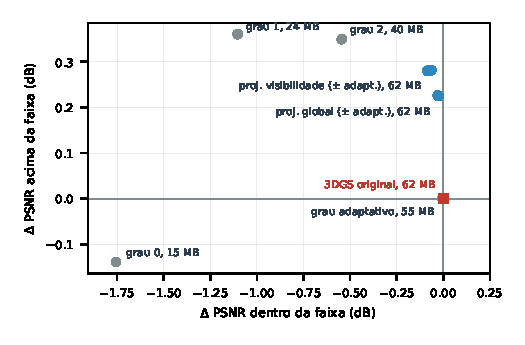
\includegraphics[width=\columnwidth]{figs/custo_qualidade_b25.pdf}
\caption{Compromisso das correções sem retreino, média das seis cenas: variação de PSNR dentro da faixa filmada (eixo horizontal) contra variação acima dela (eixo vertical), em relação ao 3DGS original. O rótulo traz o tamanho do modelo. As projeções preservam a faixa; o truncamento ganha um pouco mais fora dela, ao custo da faixa.}
\label{fig:custo}
\end{figure}

\subsection{Veículo real}

No Porsche 911 (273 mil Gaussianas, câmeras entre 0,4° e 3,8°), não há referência de cima. Medimos então quanto a projeção global altera a imagem, comparando as renderizações antes e depois dela numa volta completa em cada elevação. Na faixa filmada (2°), o PSNR entre as duas é de 49,6~dB: a mudança é imperceptível, como prevê a garantia. Acima, cai para 37,8~dB a 20°, 35,1~dB a 45° e 39,0~dB a 89°. A mudança existe, mas é pequena, e a Fig.~\ref{fig:teaser} mostra que ela não remove as manchas do teto e do capô. O comportamento é o mesmo do laboratório sintético. A ferramenta de linha de comando aplica essa projeção ao arquivo \texttt{.ply} do veículo em 0,6~s, em CPU.

% =====================================================================
\section{Discussão}\label{sec:discussao}

\textbf{Respostas às questões de pesquisa.} (QP1) A perda fora da faixa filmada é grande, 5,8~dB de cima com a faixa de 25° e 10,2~dB acima da faixa com a de 15°, e decorre da cobertura, não da dificuldade das vistas. (QP2) Ela não vem de uma geometria que piora onde nenhuma câmera olhou: silhueta e normais vistas de cima não são piores que na faixa. Em objetos reflexivos, o 3DGS reproduz as vistas filmadas com uma superfície errada e uma cor que a compensa; de cima, essa compensação deixa de valer, e reajustar com vistas de cima tanto a cor quanto a forma devolve a qualidade. (QP3) O Ref-Gaussian corrige a forma (11,6° de erro de normal de cima, contra 56,7° do 3DGS) e melhora a imagem, mas a vantagem cai de 2,1~dB na faixa para 0,7~dB de cima. O ambiente refletido de cima já havia sido observado; dentro da aparência, o que mais falta é o material das superfícies voltadas para cima, e a restrição física impede que a aparência compense o erro de geometria que resta, amplificado pelo reflexo. Com as vistas de cima, o mesmo método ganha cerca de 10~dB acima da faixa, e as iterações a mais não explicam esse ganho. (QP4) Correções aplicadas ao modelo treinado, sem informação nova, recuperam no máximo 0,4~dB. A pergunta ``cor ou geometria?'' pressupõe que as duas sejam separáveis; no 3DGS, em superfícies reflexivas, não são, e a mesma imagem filmada admite muitas combinações de forma e cor.

\textbf{Quando usar cada correção.} Os resultados indicam uma escolha por cenário. \textit{(a) Visualização de anúncios na web ou em celular}, com orçamento de memória e de banda. Quando o comprador olha sobretudo ao redor do veículo, a projeção global é a escolha: não altera a faixa filmada, reduz os reflexos inventados logo acima dela, roda em CPU sobre o arquivo final e pode ser seguida do grau adaptativo para economizar memória. Quando o tamanho pesa mais e o visualizador permite órbita livre, o truncamento para grau 2 troca 0,5~dB na faixa por 0,35~dB acima dela e 36\% de memória a menos (Tabela~\ref{tab:custo25}). Em ambos os casos, a câmera do visualizador deve ficar limitada à faixa coberta, já que nenhuma correção leve recupera a vista de topo. \textit{(b) Inspeção de veículos}, em que inventar detalhes é inaceitável: correções gerativas~\cite{wu2025difix3d,liu2024viewextrapolator} não são adequadas, e o caminho é sinalizar as vistas extrapoladas ou capturar a altura que falta; a matriz de Gram fornece essa sinalização por Gaussiana. \textit{(c) Simulação a partir de gravações de direção}, que precisa de vistas distantes da trajetória: correções leves são insuficientes, e a informação precisa vir de priors gerativos~\cite{wang2025freevs} ou de gravações com múltiplas passagens~\cite{han2025euvs}. Em todos os casos, um modelo físico como o Ref-Gaussian melhora a geometria e a imagem dentro e perto da faixa, ao custo de um treino cerca de 2,4 vezes mais longo (47 contra 20~min por cena na mesma GPU), e é a base mais promissora para incorporar conhecimento prévio sobre materiais.

\textbf{Extensão para cenas 4D automotivas.} O problema estudado aqui é mais severo em cenas dinâmicas de direção. As câmeras são fixas no veículo, cada instante é observado de um único conjunto de alturas, e os agentes em movimento são vistos de ângulos ainda mais restritos. Três elementos deste trabalho se estendem diretamente a esse caso. Primeiro, a análise de condicionamento: representações dinâmicas baseadas em Gaussianas mantêm cor por SH, inclusive variável no tempo~\cite{yan2024streetgs,wu2024gs4d}, e a matriz de Gram de cada Gaussiana pode ser calculada por janela de tempo, com os mesmos pesos de visibilidade obtidos pelo rasterizador. Segundo, o protocolo: simuladores como o CARLA~\cite{dosovitskiy2017carla} fornecem referência exata de qualquer altura, o que permite repetir o controle de cobertura e os oráculos em cenas dinâmicas, enquanto conjuntos reais com múltiplas passagens~\cite{han2025euvs} validam o resultado. Terceiro, a decomposição por oráculos, que em 4D separaria aparência, forma e movimento. Representações com primitivas explícitas são a base natural para essa extensão, porque cada Gaussiana tem posição, movimento e cor próprios, o que permite os diagnósticos por primitiva usados aqui, difíceis de aplicar a representações implícitas.

\textbf{Limitações.} (i) Os oráculos usam as vistas de referência de cima e medem um teto, não um método; como cor e forma se substituem, nenhum isola uma causa sozinho, e a conclusão decorre da combinação deles com a medida direta da geometria. (ii) O 3DGS não tem normal própria; as duas estimativas usadas (profundidade e eixo mais curto) concordam, mas são aproximações. (iii) As métricas de imagem são calculadas na imagem inteira com fundo branco, o que soma o fundo, fácil, às médias. (iv) As cenas sintéticas têm materiais muito reflexivos; veículos reais combinam pintura, vidro e plástico. (v) Cada configuração foi treinada com uma única semente; os intervalos de confiança refletem a variação entre vistas, não entre treinos. (vi) Por custo de GPU, o Ref-Gaussian foi treinado na faixa em três cenas e com 28 mil iterações; o controle com os \textit{checkpoints} do modelo completo indica que as iterações pesam pouco, mas o cronograma escalado não é idêntico ao original. (vii) A garantia da projeção vale nas direções de treino; com a faixa de 15°, a versão por visibilidade piora as vistas de teste da própria faixa, e só a global permanece neutra. (viii) Os oráculos do Ref-Gaussian usam 1000 passos, contra 3000 nos do 3DGS, e mantêm a malha usada na luz indireta; seus ganhos são, portanto, limites inferiores do que cada componente poderia recuperar.

\textbf{Trabalhos futuros.} (i) Completar a decomposição do Ref-Gaussian com um oráculo de geometria (posições, formas e normais), que mediria quanto do erro de cima vem do desvio residual das normais amplificado pelo reflexo. (ii) Aprender um prior de materiais com objetos sintéticos observados de todos os ângulos e usá-lo dentro do Ref-Gaussian, que já tem geometria e ambiente corretos e onde o material é a componente que mais falta. (iii) Repetir o protocolo em cenas dinâmicas de direção, com o CARLA e com conjuntos reais de múltiplas passagens. (iv) Comparar, no mesmo protocolo, correções gerativas como Difix3D+~\cite{wu2025difix3d}, medindo também quanto elas inventam. (v) Usar a matriz de Gram como mapa de confiança por Gaussiana, para guiar a captura e sinalizar vistas extrapoladas. (vi) Repetir os treinos com várias sementes e medir as métricas só nos pixels do objeto.

% =====================================================================
\section{Conclusão}\label{sec:conclusao}

Este trabalho mediu, num cenário controlado e com foco no domínio automotivo, o que acontece quando um modelo 3DGS treinado com vistas numa faixa estreita de elevação é visto de cima. A perda média é de 5,8~dB de PSNR com a faixa de 25° e cresce com faixas mais estreitas. A análise da matriz de Gram mostra que uma faixa estreita deixa a maior parte dos coeficientes de cor indeterminada, e uma projeção sem treino, com garantia de alterar pouco as direções observadas, remove esses coeficientes em menos de 1~s. Ela melhora as vistas logo acima da faixa (+0,28~dB, 84\% das vistas), mas quase nada de cima. Oráculos e a medida direta da geometria mostram o motivo: a geometria vista de cima não é pior que a da faixa, mas está errada em todas as alturas, e o modelo reproduz as vistas filmadas compensando-a com a cor. O Ref-Gaussian, modelo de reflexão baseado em física, corrige a forma (12° de erro de normal de cima, contra 57°), mas perde de cima tanto quanto o 3DGS, embora o ambiente refletido de cima já tivesse aparecido no treino. Oráculos por componente mostram que, na aparência dele, o que mais falta é o material das superfícies vistas só de raspão, e que a restrição física, que garante a forma correta, impede a aparência de compensar o erro de normal que resta. Com as vistas de cima, o mesmo método ganha cerca de 10~dB, e o controle por \textit{checkpoints} mostra que esse ganho não vem das iterações. Fora do ângulo filmado falta informação, não ajuste. Correções leves têm lugar em visualização com orçamento de memória, desde que acompanhadas da limitação do ponto de vista; vistas distantes exigem captura adicional ou conhecimento prévio. A extensão natural é o caso dinâmico das gravações de direção, em que a cobertura limitada é a regra.
